% $$$$$$\  $$\                            $$\     
% $$  __$$\ $$ |                           $$ |    
% $$ /  \__|$$$$$$$\   $$$$$$\   $$$$$$\ $$$$$$\   
% $$ |      $$  __$$\ $$  __$$\ $$  __$$\\_$$  _|  
% $$ |      $$ |  $$ |$$$$$$$$ |$$$$$$$$ | $$ |    
% $$ |  $$\ $$ |  $$ |$$   ____|$$   ____| $$ |$$\ 
% \$$$$$$  |$$ |  $$ |\$$$$$$$\ \$$$$$$$\  \$$$$  |
%  \______/ \__|  \__| \_______| \_______|  \____/
\chapter{Connected Spaces and Sets}
\section{Definition and Theorems}
\begin{defbox}
    \begin{definition}
        A {\color{mathobj}topological space} \((X, \mathcal{O})\) is said to be {\color{maththen}connected}, if one of the following {\color{mathrem}equivalent} conditions is met.
        \begin{enumerate}
            \item \(X\) is \textbf{not} a {\color{mathif}union} of two {\color{mathif}nonempty}, {\color{mathif}disjoint}, and {\color{mathif} open subsets}, i.e. there are no open subsets \(A, B \in \mathcal{O}\) with \(A, B \neq \varnothing\) and \(A \cap B = \varnothing\) such that \(A \sqcup B = X\).
            \item The \textbf{only} {\color{mathif}subsets} of \(X\) that are \textbf{both} {\color{mathif}open} and {\color{mathif}closed} ({\color{mathrem}clopen}) are the empty set \(\varnothing\) and the entire set \(X\), i.e. if \(A \subset X\) is a subset with \(A \in \mathcal{O}\) and \(X \setminus A \in \mathcal{O}\), then \(A = \varnothing\) or \(A = X\).
            \item The \textbf{only} {\color{mathif}subsets} of \(X\) with empty {\color{mathif}boundary} are the emptyset \(\varnothing\) and the entire set \(X\).
            \item All {\color{mathif}continuous} maps from \(X\) to the two point space \(\{0, 1\}\) endowed with the {\color{mathif}discrete} topology is {\color{mathif}constant}. 
        \end{enumerate}
        A {\color{mathobj}subset} of \(X\) is {\color{maththen}connected} if it is a {\color{mathif}connected space} when viewed as a {\color{mathif}subspace} of \(X\).
    \end{definition}
\end{defbox}

\begin{thmbox}
    \begin{lemma}
        Any {\color{mathif}interval} \(I \subset \mathbb{R}\) is {\color{maththen}connected}.
    \end{lemma}
\end{thmbox}
%
\begin{thmbox}
    \begin{lemma}
        Let \(X\) and \(Y\) be {\color{mathif}topological spaces} and \(f: X \longrightarrow Y\) a {\color{mathif}continuous function}. If \(X\) is {\color{mathif}connected}, then \(f(X) \subset Y\) is {\color{maththen}connected}.
    \end{lemma}
\end{thmbox}
%
\begin{defbox}
    \begin{definition}
        A connected component of a topological space is a maximally connected subset \(X_0 \subseteq X\), i.e. \(X_0\) connected and for all \(X_0 \subsetneq X_1\) then \(X_1\) is not connected.
    \end{definition}
\end{defbox}
%
\begin{thmbox}
    \begin{proposition}
        Connected components are closed subsets.
    \end{proposition}
\end{thmbox}
%
\begin{thmbox}
    \begin{lemma}[Lemma 11]
        Let \(X\) be connected and \(f: X \longrightarrow Y\) and locally constant, i.e. for all \(x \in X\) there exists a \(U_x \in \mathcal{O}_X\), \(x \in U_x\) such that \(f\) restricted on \(U_x\) is identical to \(f(x)\)., then \(f\) is constant.
    \end{lemma}
\end{thmbox}
%
\begin{defbox}
    \begin{definition}
        \(X\) is said to be {\color{maththen}path connected}, if for every pair of points \(x\) and \(x_0\) in \(X\) there is a continuous map (called path) \(\gamma: [0, 1] \longrightarrow X\) with \(\gamma(0) = x_0\) and \(\gamma(1) = x\).
    \end{definition}
\end{defbox}
%
\begin{thmbox}
    \begin{lemma}
        If \(X\) is path connected, then it is also connected.
    \end{lemma}
\end{thmbox}
\newpage
% $$$$$$$\                                 $$$$$$\  
% $$  __$$\                               $$  __$$\ 
% $$ |  $$ | $$$$$$\   $$$$$$\   $$$$$$\  $$ /  \__|
% $$$$$$$  |$$  __$$\ $$  __$$\ $$  __$$\ $$$$\     
% $$  ____/ $$ |  \__|$$ /  $$ |$$ /  $$ |$$  _|    
% $$ |      $$ |      $$ |  $$ |$$ |  $$ |$$ |      
% $$ |      $$ |      \$$$$$$  |\$$$$$$  |$$ |      
% \__|      \__|       \______/  \______/ \__|
\section{Proofs, Remarks, and Examples}
\begin{defbox}
    \begin{definition}
        A {\color{mathobj}topological space} \((X, \mathcal{O})\) is said to be {\color{maththen}connected}, if one of the following {\color{mathrem}equivalent} conditions is met.
        \begin{enumerate}
            \item \(X\) is \textbf{not} a {\color{mathif}union} of two {\color{mathif}nonempty}, {\color{mathif}disjoint}, and {\color{mathif} open subsets}, i.e. there are no open subsets \(A, B \in \mathcal{O}\) with \(A, B \neq \varnothing\) and \(A \cap B = \varnothing\) such that \(A \sqcup B = X\).
            \item The \textbf{only} {\color{mathif}subsets} of \(X\) that are \textbf{both} {\color{mathif}open} and {\color{mathif}closed} ({\color{mathrem}clopen}) are the empty set \(\varnothing\) and the entire set \(X\), i.e. if \(A \subset X\) is a subset with \(A \in \mathcal{O}\) and \(X \setminus A \in \mathcal{O}\), then \(A = \varnothing\) or \(A = X\).
            \item The \textbf{only} {\color{mathif}subsets} of \(X\) with empty {\color{mathif}boundary} are the emptyset \(\varnothing\) and the entire set \(X\).
            \item All {\color{mathif}continuous} maps from \(X\) to the two point space \(\{0, 1\}\) endowed with the {\color{mathif}discrete} topology is {\color{mathif}constant}. 
        \end{enumerate}
        A {\color{mathobj}subset} of \(X\) is {\color{maththen}connected} if it is a {\color{mathif}connected space} when viewed as a {\color{mathif}subspace} of \(X\).
    \end{definition}
\end{defbox}
\begin{proof}
    We verify the equivalence of the different definitions. So, let \((X, \mathcal{O})\) be a topological space.
    \begin{itemize}
        \item ``\textit{1. \(\Rightarrow\) 2.}'': Assume that \(X\) is not a union of two nonempty, disjoint, and open subsets. Fix a subset \(A \in X\) that is clopen. If \(A\) is neither the empty set nor \(X\), then \(X \setminus A\) is also not the empty set nor \(X\). Clearly, \(A\) and \(X \setminus A\) are disjoint and they are also open because \(A\) is clopen. But \(A \sqcup B = X\), so our assumption was absurd. It must be that \(A = \varnothing\) or \(A = X\).
        \item ``\textit{2. \(\Rightarrow\)} 1.'': Now let the only clopen set contained in \(X\) be the empty set or \(X\) itself. Assume there are \(A, B \in \mathcal{O}\) with \(A, B \neq \varnothing\) and \(A \cap B = \varnothing\) such that \(A \sqcup B = X\). Then, \(A\) is open, but also closed because \(X \setminus A = B\) is open. Furthermore, \(A\) is not empty and since \(B\) is also not empty, \(A \neq X\). Hence our assumption was wrong and there no nonempty, disjoint, and open subsets \(A\) and \(B\) such that \(A \sqcup B = X\).
        \item ``\textit{2. \(\iff\) 3.}'': This is one of the properties of clopen subsets and was proven in remark XXX.
        \item ``\textit{1. \(\Rightarrow\) 4.}'': Let \(X\) not be a union of two nonempty, disjoint, and open subsets. Assume there exists a continuous function \(f: X \longrightarrow \{0, 1\}\) with regards to the discrete topology that is not constant. Then, \(f^{-1}(\{0\})\) and \(f^{-1}(\{1\})\) are nonempty sets that are also disjoint. Since \(f\) is continuous, these are also open subsets. But we also have \(f^{-1}(\{0\}) \sqcup f^{-1}(\{1\}) = X\).
        \item ``\textit{4. \(\Rightarrow\) 1.}'': Let all continuous functions with regards to the discrete topology be constant. Assume there are two nonempty, disjoint, and open subsets \(A, B \in \mathcal{O}\) such that \(A \sqcup B = X\). Define \(f: X \longrightarrow \{0, 1\}\) as \(f(A) = 0\) and \(f(B) = 1\). This definition is well-defined because \(A, B \in \mathcal{O}\) are nonempty, disjoint, and \(A \sqcup B = X\). \(f\) is also continuous as the preimage of \(\{0\}\) and \(\{1\}\) are \(A\) and \(B\) respectively which are open subsets. Hence our assumption was wrong.
    \end{itemize}
\end{proof}
\begin{thmbox}
    \begin{lemma}
        Any {\color{mathif}interval} \(I \subset \mathbb{R}\) is {\color{maththen}connected}.
    \end{lemma}
\end{thmbox}
%
\begin{proof}
    Fix an interval \(I \subset \mathbb{R}\), and let \(A, B \subset \mathbb{R}\) be two nonempty, open and disjoint subsets such that \(A \sqcup B = I\). Moreover, let \(a \in A\) and \(b \in B\) and assume without loss of generality that \(a < b\). If we set
    \begin{align}
        s := \inf \makeset{x \in B}{a < x} \text{,}
    \end{align}
    then \(s \in I\) because \(s\) is between \(a\) and \(b\) and we have \([a, b] \subset I\).

    Now, on one side, we have \(s \in \mathrm{cl}(B)\) and since the complement of \(B\) is an open subset \(A\), so \(B = \mathrm{cl}(B)\). It is therefore \(x \in B\).
    
    But we also have \(s \in A\) because the infimum cannot be contained in an open set, but \(s \in I = A \sqcup B\).
\end{proof}
%
\begin{thmbox}
    \begin{lemma}
        Let \(X\) and \(Y\) be {\color{mathif}topological spaces} and \(f: X \longrightarrow Y\) a {\color{mathif}continuous function}. If \(X\) is {\color{mathif}connected}, then \(f(X) \subset Y\) is {\color{maththen}connected}.
    \end{lemma}
\end{thmbox}
%
\begin{proof}
    Let \(f(X) = A \sqcup B\) with \(A\) and \(B\) being two open disjoint sets. \(f^{-1}(A)\) and \(f^{-1}(B)\) are open since \(f\) is continuous. We also have \(f^{-1}(A) \cap f^{-1}B = f^{-1}(A \cap B) = \varnothing\) so \(f^{-1}(A) = \varnothing\) or \(f^{-1}(B) = \varnothing\), so \(A = \varnothing\) or \(B = \varnothing\) and we are done.
\end{proof}
%
\begin{rembox}
    \begin{remark}
        The two lemma above are handy to show that images of functions are connected.
    \end{remark}
\end{rembox}
%
\begin{example}
    The general linear group \(\mathrm{GL}_n(K)\) for a field \(K\) and \(n \in \mathbb{N}\) is not connected for \(K = \mathbb{R}\) and \(K = \mathbb{C}\).
\end{example}
%
\begin{proof}
    % what to do in the case of n = 0?
    Define the following partition of \(\mathrm{GL}_n(\mathbb{K})\)
    \begin{align*}
        A &:= \makeset{M \in \mathrm{Mat}_{n \times n}(\mathbb{K})}{\mathrm{det}(M) > 0} \\
        B &:= \makeset{M \in \mathrm{Mat}_{n \times n}(\mathbb{K})}{\mathrm{det}(M) < 0} \text{,}
    \end{align*}
    then, \(A\) and \(B\) are disjoint, nonempty, and \(\mathrm{GL}_n(\mathbb{K}) = A \sqcup B\). We show that \(A\) and \(B\) are open sets.

    The determinant function \(\mathrm{det}: \mathrm{Mat}_{n \times n}(\mathbb{K}) \longrightarrow \mathbb{C}\) is continuous because it is a multivariate polynomial. \(\mathbb{R}^+\) is an interval, therefore open, and so \(\mathrm{det}^{-1}(\mathbb{R}^+) = A\) is also open. Similary \(B\) is an open subset. Hence \(\mathrm{GL}_n(\mathbb{K})\) is not connected.
\end{proof}
%
\begin{rembox}
    \begin{remark}
        In the proof above, the topology of \(\mathrm{Mat}_{n \times n}(\mathbb{K})\) matters because the continuity of the determinant function depends on the underlying topology.
    \end{remark}
\end{rembox}
%
\begin{defbox}
    \begin{definition}
        A connected component of a topological space is a maximally connected subset \(X_0 \subseteq X\), i.e. \(X_0\) connected and for all \(X_0 \subsetneq X_1\) then \(X_1\) is not connected.
    \end{definition}
\end{defbox}
%
\begin{example}
    For \(\mathbb{Q} \subset \mathbb{R}\) the connected components are points and those are not open.
\end{example}
%
\begin{thmbox}
    \begin{proposition}
        Connected components are closed subsets.
    \end{proposition}
\end{thmbox}
%

\begin{proof}
    Locally constant implies continuous with regards to the discrete topology on \(Y\). Let \(x \in X\), \(X = f^{-1}(f(x)) \cup f^{-1}(Y \setminus \{f(x)\})\) is a disjoint union and since \(X\) is connected \(f^{-1}(Y \setminus \{f(x)\}) = \varnothing\). Conclude \(f\) is identical to \(f(x)\).
\end{proof}

\textbf{Application:} \(f: X \longrightarrow \{0, 1\}\), \(X\) is connected, \(f\) locally constant, there is a \(x \in X\) such that \(f(x) = 1\), then \(f\) is identical to \(1\).

\begin{proof}
    Let \(A\) and \(B\) two disjoint open sets such that \(A \sqcup B = X\), and let \(a \in A\) and \(b \in B\). Let \(\gamma: [0, 1] \longrightarrow X\) be continuous path with \(\gamma(0) = x_0\) and \(\gamma(1) = x_1\). We have that \(\gamma^{-1}\)
\end{proof}

\newpage
% $$\   $$\            $$\                         
% $$$\  $$ |           $$ |                        
% $$$$\ $$ | $$$$$$\ $$$$$$\    $$$$$$\   $$$$$$$\ 
% $$ $$\$$ |$$  __$$\\_$$  _|  $$  __$$\ $$  _____|
% $$ \$$$$ |$$ /  $$ | $$ |    $$$$$$$$ |\$$$$$$\  
% $$ |\$$$ |$$ |  $$ | $$ |$$\ $$   ____| \____$$\ 
% $$ | \$$ |\$$$$$$  | \$$$$  |\$$$$$$$\ $$$$$$$  |
% \__|  \__| \______/   \____/  \_______|\_______/
\section{Exercises and Notes}
% exercise
\subsection{Connectedness}
\begin{thmbox}
    \begin{lemma}
    If \((X, \mathcal{O_X})\) and \((Y, \mathcal{O}_Y)\) are two connected topological spaces, then their product \(X \times Y\) with the product topology \(\mathcal{O}_{X \times Y}\)is also connected.
    \end{lemma}
\end{thmbox}
%
\begin{proof}
    We will use the definition that all continuous maps from \(X \times Y\) to \(\{0, 1\}\) endowed with the discrete topology must be constant. Fix a continuous \(f: X \longrightarrow \{0, 1\}\).
    
    First, consider the image \(f(\{x\} \times Y)\) with \(x \in X\). Assume \(f\) is not constant on \(\{x\} \times Y\), then \(f(\{x\} \times Y) = \{0, 1\}\). So we have the preimages \(f^{-1}(\{0\}) = \{x\} \times U\) and \(f^{-1}(\{1\}) = \{x\} \times V\) with \(U, V \subset Y\), \(U, V \neq \varnothing\), and \(U \cap V = \varnothing\). Because \(f\) is continuous, \(U\) and \(V\) must also be open. This would however mean that \(U \sqcup V = Y\) and \(Y\) would not be connected, therefore, \(f\) is constant on \(\{x\} \times Y\). Similary, we get that \(f\) is constant on \(X \times \{y\}\) for all \(y \in Y\).

    Let \((x, y) \in X \times Y\) and \((x', y') \in X \times Y\) be two arbitary points. We have \(f(x, y) = f(x, y')\) because \(f\) is constant on \(\{x\} \times Y\) and similary \(f(x, y') = f(x', y')\) because \(f\) is constant on \(X \times \{y\}\). Putting everything together, it is \(f(x, y) = f(x',y')\), therefore all continuous \(f: X \times Y \longrightarrow \{0, 1\}\) are constant.
\end{proof}
%
\begin{example}
    Clearly, the union of two connected sets need not be connected. Take for example \([0, 1] \subset \mathbb{R}\) and \([2, 3] \subset \mathbb{R}\). Their union \([0, 1] \cup [2, 3]\) is not connected.

    Set difference of connected sets are also not necessarily connected, e.g. \([0, 2] \subset \mathbb{R}\) and \(\{1\} \subset \mathbb{R}\) are connected, but \([0, 2] \setminus \{1\} = [0, 1) \cup (1, 2]\) is not.

    More interestingly, the intersection of two connected sets also need not be connected. Consider the unit circle around the origin \(S^1 = \makeset{(x, y)}{x^2 + y^2 = 1}\) and another unit circle around \((1, 0)\) \(A := \makeset{(x, y)}{(x-1)^2 + y^2 = 1}\). They are both connected, but their intersection is a two point set
    \begin{equation*}
        \set{\left(\frac{1}{2}, \frac{1}{2}\sqrt{3}\right),\, \left(\frac{1}{2}, -\frac{1}{2}\sqrt{3}\right)}
    \end{equation*}
    which is not connected.
\end{example}
%
%
\begin{thmbox}
    \begin{proposition}
        \begin{enumerate}
            \item Every trivial topological space is connected.
            \item Every discrete topological space with at least two elements is disconnected.
            \item Trivially, every singleton set and the empty set are connected spaces vacuously.
        \end{enumerate}
    \end{proposition}
\end{thmbox}
%
\begin{proof}
    \begin{enumerate}
        \item Let \(X\) be an arbitary set and \(\mathcal{O} = \set{\varnothing, X}\) be the trivial topology. If \(S \subset X\) is a clopen subset, then it is trivially either \(\varnothing\) or \(X\), therefore, \(X\) is connected.
        \item Let \(X\) be a set containing more than one element and \(\mathcal{O} = \mathcal{P}(X)\) be the discrete topology of \(X\). Let \(A \subset X\) be a nonempty proper subset, then \(B := X \setminus A\) is also not empty. Both are open subsets, but \(A \sqcup B = X\), so \(X\) is not connected.
    \end{enumerate}
\end{proof}

\subsection{Path-Connectedness}
\begin{example}
    Connectedness does not imply path-connectedness. Let \(\mathbb{R}^2\) be endowed with the Euclidean topology and consider 
    \begin{equation*}
        X = \makeset{\left(x, \sin\left(\frac{1}{x}\right)\right)}{x > 0} \cup \left(\,\{0\} \times [-1, 1]\,\right) \subset \mathbb{R}^2 \text{.}
    \end{equation*}
    %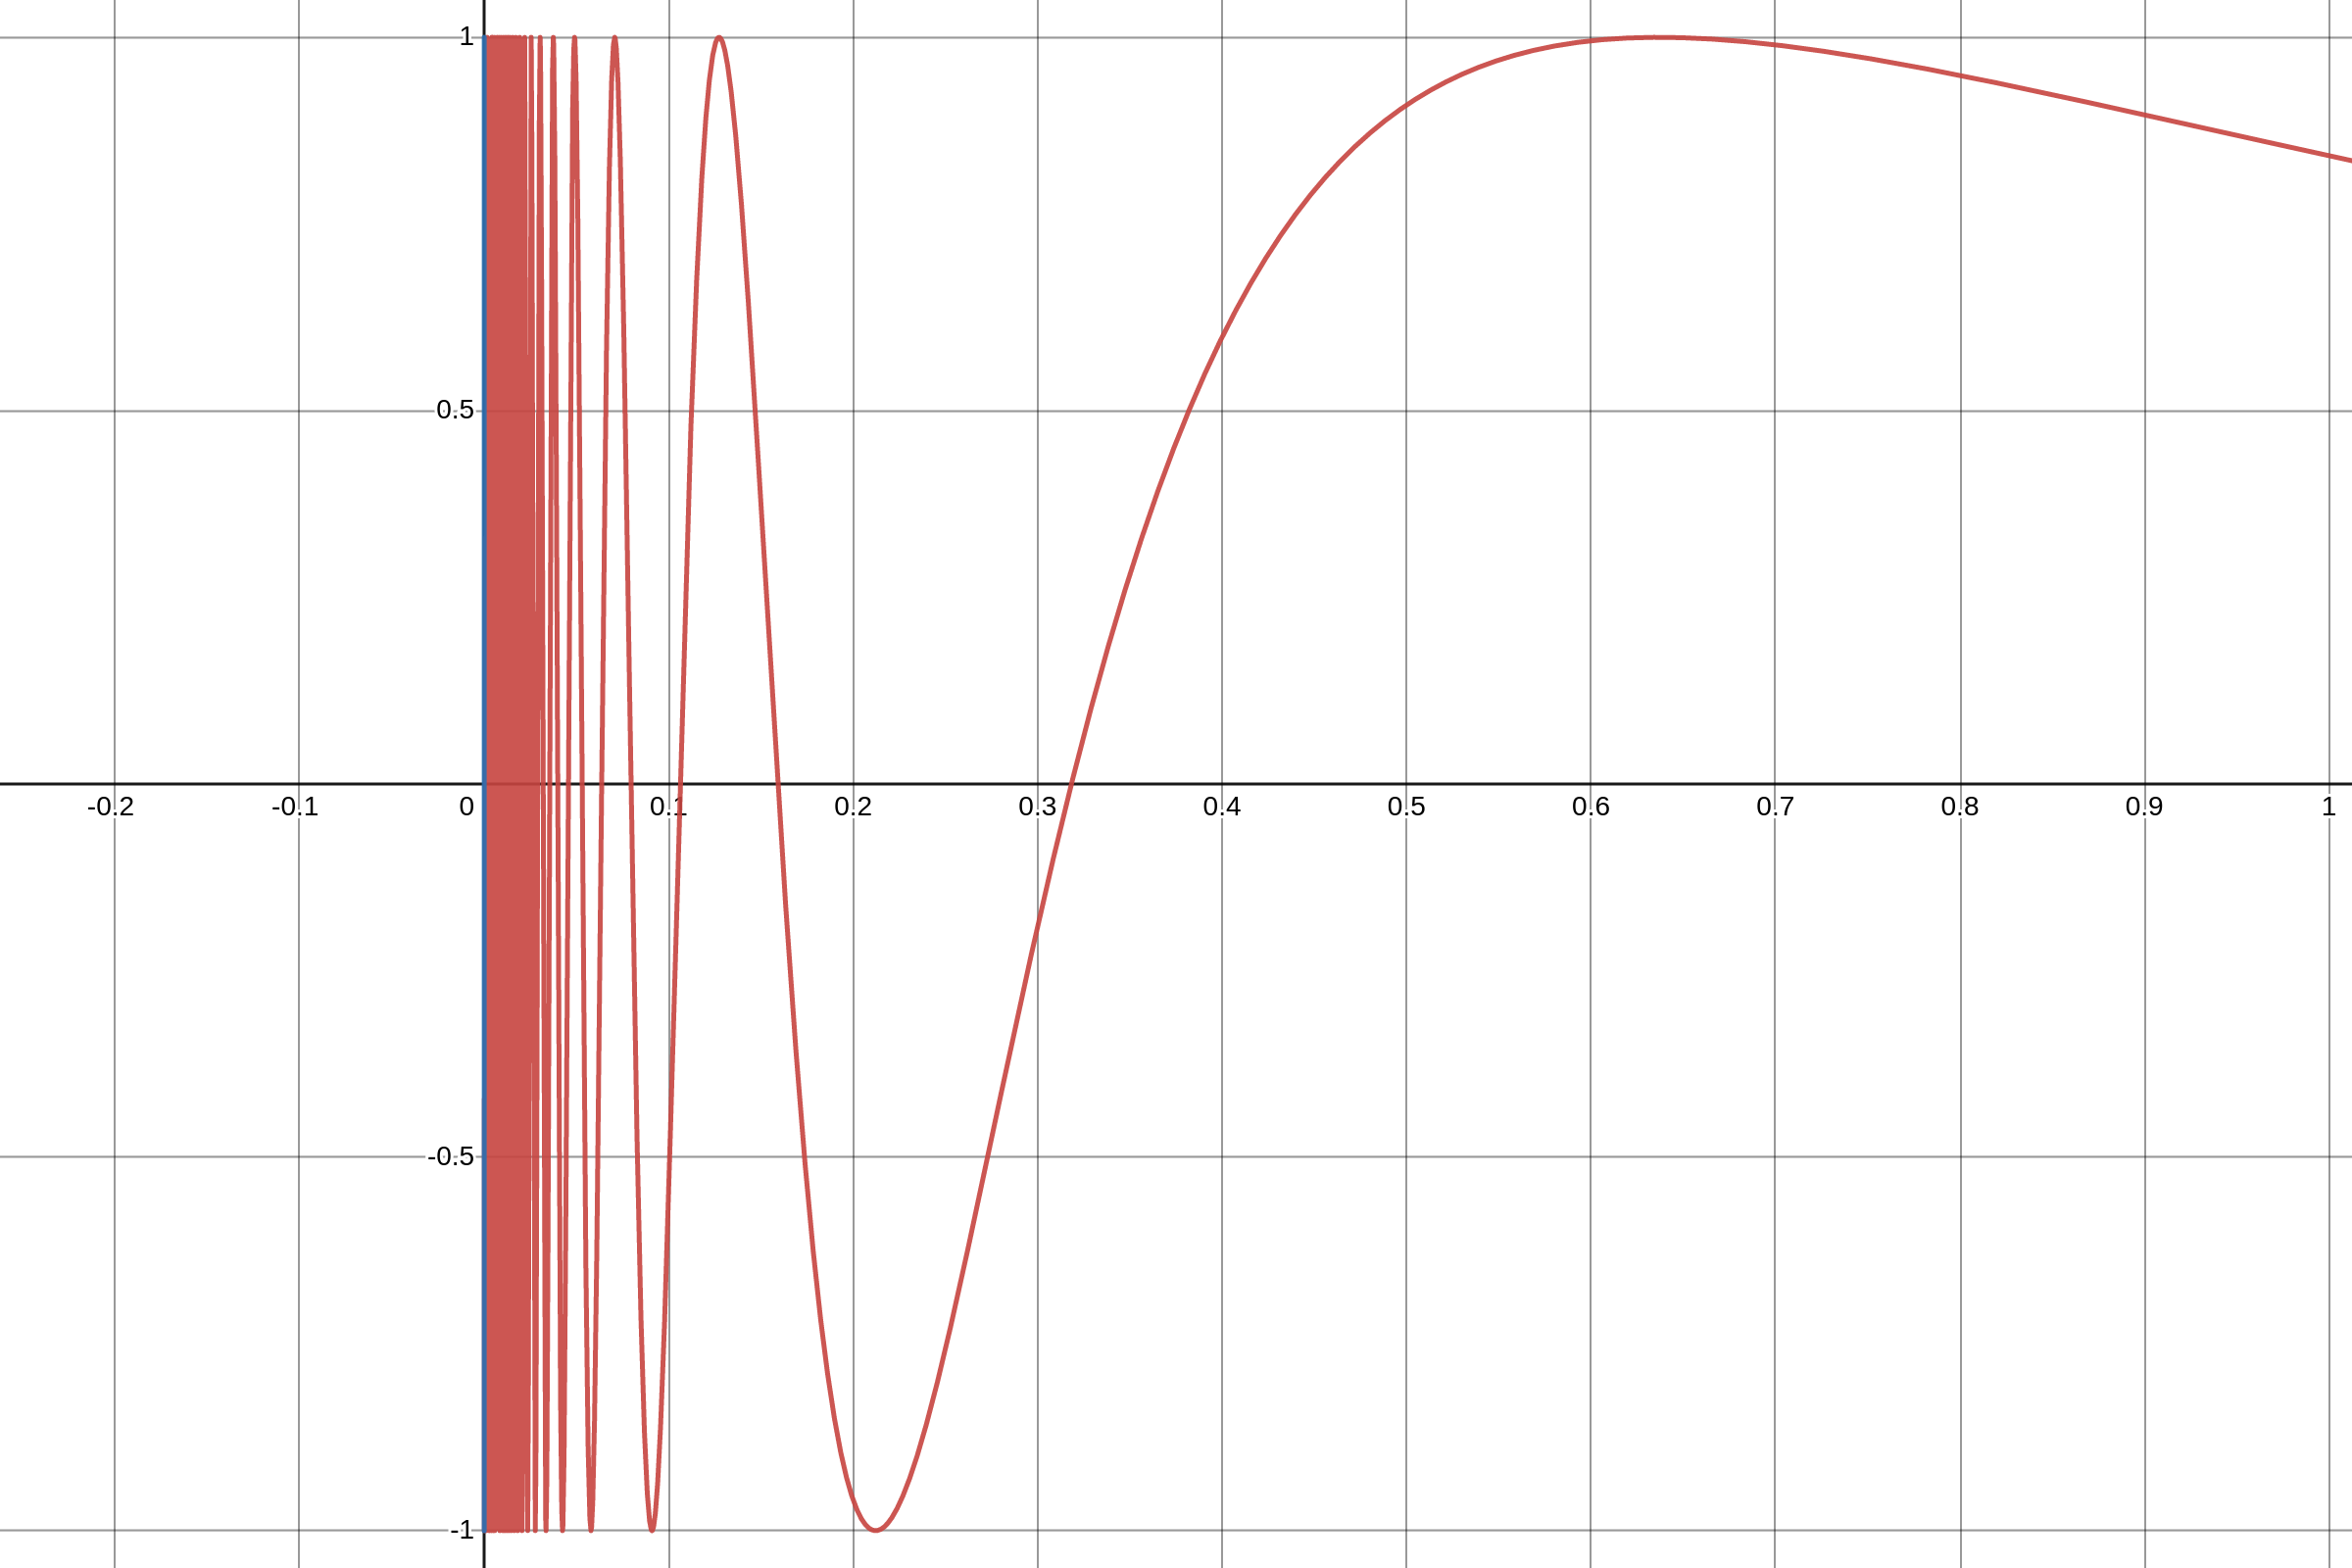
\includegraphics[width=0.5\textwidth]{image/desmos-graph.png}
    and see figure XXX. \(X\) is connected, but it is not path-connected.
\end{example}
\begin{proof}
    Denote
    \begin{equation*}
        A := \makeset{\left(x, \sin\left(\frac{1}{x}\right)\right)}{x > 0} \qquad B := \{0\} \cup [-1, 1] \text{,}
    \end{equation*}
    then \(X = A \sqcup B\).
    \begin{enumerate}
        \item First, define \(f: \mathbb{R}^+ \longrightarrow \mathbb{R}^2\) as
        \begin{equation*}
            f(x) := \left(x,\, \sin\left(\frac{1}{x}\right)\right) \text{.}
        \end{equation*}
        \(f\) is continuous, \(\mathbb{R}^+\) is an interval, therefore connected, so \(f(\mathbb{R}^+) = A\) is connected. On the other hand, \(\{0\}\) and \([-1, 1]\) are connected and so is their product \(B\).
        
        Assume there is a clopen subset \(S \subset X\) that is not empty. Without loss of generality, we have that \((0, 0) \in U\) (otherwise, consider the complement of \(U\) which also must be clopen). Since \(A\) is clopen in \(A\), the intersection \(A \cap U\) must also be clopen in \(A\), but \(A\) is connected, so \(A\) is contained in \(U\).

        Moreover, the closure of \(A\) is also contained in \(U\). So there is an \(\epsilon > 0\) such that the ball \(B(p, \epsilon)\) that contains \((0, 0)\) is in \(U\). I got lazy to go into the details, but this ball contains a point of \(B\). Follow the same reason as above.
        \item 
    \end{enumerate}
\end{proof}